%% IMPORTANT NOTICE:
%% For the copyright see the source file.
%% 
%% Any modified versions of this file must be renamed
%% with new filenames distinct from sample-sigplan.tex

%% The first command in your LaTeX source must be the \documentclass command.
\documentclass[manuscript, screen]{acmart}
%%
%% \BibTeX command to typeset BibTeX logo in the docs
\AtBeginDocument{%
  \providecommand\BibTeX{{%
    \normalfont B\kern-0.5em{\scshape i\kern-0.25em b}\kern-0.8em\TeX}}}
    
%% Allows images to be inserted:
\usepackage{graphicx}
\graphicspath{ {./images/} }
\usepackage{wrapfig}

% \usepackage[table]{color}
% \usepackage{multirow}
% \usepackage{array}
% \usepackage{makecell}
% \usepackage{todonotes}
% \usepackage{float}
% \raggedbottom





%% Rights management information.  This information is sent to you
%% when you complete the rights form.  These commands have SAMPLE
%% values in them; it is your responsibility as an author to replace
%% the commands and values with those provided to you when you
%% complete the rights form.
\setcopyright{acmcopyright}
\copyrightyear{2021}
\acmYear{2021}
%\acmDOI{10.1145/1122445.1122456}

%% These commands are for a PROCEEDINGS abstract or paper.
\acmConference[Woodstock '18]{Woodstock '18: ACM Symposium on Neural
  Gaze Detection}{June 03--05, 2018}{Woodstock, NY}
\acmBooktitle{Woodstock '18: ACM Symposium on Neural Gaze Detection,
  June 03--05, 2018, Woodstock, NY}
\acmPrice{15.00}
\acmISBN{978-1-4503-XXXX-X/18/06}

%% Submission ID.
%% Use this when submitting an article to a sponsored event. You'll
%% receive a unique submission ID from the organizers
%% of the event, and this ID should be used as the parameter to this command.
%%\acmSubmissionID{123-A56-BU3}

%% end of the preamble, start of the body of the document source.
\begin{document}
%% The "title" command has an optional parameter,
%% allowing the author to define a "short title" to be used in page headers.
\title{Monster Munch, A Mobile Application for Nutritional Engagement}

%% The "author" command and its associated commands are used to define the authors and their affiliations.
%% Of note is the shared affiliation of the first two authors, and the
%% "authornote" and "authornotemark" commands
%% used to denote shared contribution to the research.
\author{Author1}
\authornote{Both authors contributed equally to this research.}
\email{}
\orcid{}
\author{Author2}
\authornotemark[1]
\email{}
\affiliation{%
  \institution{}
  \streetaddress{}
  \city{}
  \state{}
  \postcode{}
}

\author{Lars Th{\o}rv{\"a}ld}
\affiliation{%
  \institution{The Th{\o}rv{\"a}ld Group}
  \streetaddress{1 Th{\o}rv{\"a}ld Circle}
  \city{Hekla}
  \country{Iceland}}
\email{larst@affiliation.org}

\author{Valerie B\'eranger}
\affiliation{%
  \institution{Inria Paris-Rocquencourt}
  \city{Rocquencourt}
  \country{France}
}

\author{Aparna Patel}
\affiliation{%
 \institution{Rajiv Gandhi University}
 \streetaddress{Rono-Hills}
 \city{Doimukh}
 \state{Arunachal Pradesh}
 \country{India}}

\author{Huifen Chan}
\affiliation{%
  \institution{Tsinghua University}
  \streetaddress{30 Shuangqing Rd}
  \city{Haidian Qu}
  \state{Beijing Shi}
  \country{China}}

% \author{Charles Palmer}
% \affiliation{%
%   \institution{Palmer Research Laboratories}
%   \streetaddress{8600 Datapoint Drive}
%   \city{San Antonio}
%   \state{Texas}
%   \postcode{78229}}
% \email{cpalmer@prl.com}

\renewcommand{\shortauthors}{Author1 and Author2, et al.}

%%
%% The abstract is a short summary of the work to be presented in the
%% article.


%%
%% The code below is generated by the tool at http://dl.acm.org/ccs.cfm.
%% Please copy and paste the code instead of the example below.
%%
\begin{CCSXML}
<ccs2012>
 <concept>
  <concept_id>10010520.10010553.10010562</concept_id>
  <concept_desc>Computer systems organization~Embedded systems</concept_desc>
  <concept_significance>500</concept_significance>
 </concept>
 <concept>
  <concept_id>10010520.10010575.10010755</concept_id>
  <concept_desc>Computer systems organization~Redundancy</concept_desc>
  <concept_significance>300</concept_significance>
 </concept>
 <concept>
  <concept_id>10010520.10010553.10010554</concept_id>
  <concept_desc>Computer systems organization~Robotics</concept_desc>
  <concept_significance>100</concept_significance>
 </concept>
 <concept>
  <concept_id>10003033.10003083.10003095</concept_id>
  <concept_desc>Networks~Network reliability</concept_desc>
  <concept_significance>100</concept_significance>
 </concept>
</ccs2012>
\end{CCSXML}

\ccsdesc[500]{Computer systems organization~Embedded systems}
\ccsdesc[300]{Computer systems organization~Redundancy}
\ccsdesc{Computer systems organization~Robotics}
\ccsdesc[100]{Networks~Network reliability}

%%
%% Keywords. The author(s) should pick words that accurately describe
%% the work being presented. Separate the keywords with commas.
\keywords{avatars, nutritional engagement, macronutrients, meal photos, crowdsourcing, community board}


%%
%% This command processes the author and affiliation and title
%% information and builds the first part of the formatted document.
\maketitle


Nutrition is a crucial part of healthy living, however, individuals often struggle to understand and make healthy choices. Past HCI work, particularly in health, has shown the power of gamification in promoting engagement with and understanding of complex information. Leveraging gamification techniques (avatars and crowdsourced feedback) to help people engage with nutrition, we developed Monster Munch, a mobile application where users help monster avatars achieve a particular health goal (e.g., lose weight) by selecting crowdsourced ``in-the-wild'' meals to feed them. We piloted Monster Munch (N=68) and found users' confidence assessing macronutrients increased after using the app. Strong player-avatar-identification (PAID) and increased utilization of the crowdsourced community board were related to users' enjoyment of the app. Interestingly, lower PAID predicted greater recall of nutrition information, independent of prior nutrition knowledge. Findings suggest PAID may be an important mechanism in learning and highlights how fun, lightweight tools can prompt reflection and recall.




  

\section{Introduction}
Unhealthy eating contributes to the obesity epidemic in the United States, which affects 12 million American adolescents and 38\% of adults \cite{trustforamericashealth,cdc2015,cdc2020}. 
%The estimated annual medical cost of obesity exceeded \$147 billion dollars in 2008 [PLACE UPDATED REF]~\cite{ }. 
While there are many factors that contribute to unhealthy eating, past work highlights low nutritional literacy as a key factor, in particular limited ability to accurately estimate nutritional composition (i.e., macronutrient content) of meals ~\cite{kindig2004health}. 
While estimating the nutritional composition of meals is crucial for health management and preventing undesired health consequences (especially for individuals with chronic conditions), previous studies show doing so is a considerable challenge. For example, individuals from low-literacy backgrounds often have difficulty interpreting Nutrition Fact labels, leading to miscalculation of the amount of consumed nutrients \cite{chaudry2013formative,huizinga2009literacy,rothman2006patient}. Even professional dietitians~\cite{chandon2007obesity} and healthy eaters often underestimate calories in meals~\cite{chandon2007biasing}. Complex meals such as salads and dressings with many components add another layer of difficulty with nutritional assessment~\cite{noronha2011platemate}.


Due to the difficulty in nutritional estimation, as well as the huge user burden with many self-tracking and food journaling apps, people develop short-lived commitments to these tools and often are fatigued leading to complete abandonment of the app and self-tracking habits~\cite{choe2014understanding,Cordeiro:2015:RMF:2702123.2702154,cordeiro2015barriers,epstein2016crumbs,mattila2008mobile}. A variety of \textit{interactive, gamified solutions} have emerged to help individuals engage with nutrition information easily, promote meal tracking and behavior change, and improve learning. Noting the high burden of tracking ingredients and meals many users report~\cite{desai2019personal}, some solutions automate the process of nutrition logging 
through bar code scanning and ingredient selection from existing databases ~\cite{beijbom2015menu,bomfim2018pirate,bomfim2020food,siek2009evaluation}, lightweight social interactive challenges~\cite{Cordeiro:2015:RMF:2702123.2702154,epstein2016crumbs},
computational image analysis~\cite{anthimopoulos2015computer,kong2012dietcam,rhyner2016carbohydrate,zhang2015snap,zhu2010use}, crowdsourcing~\cite{mamykina2011examining,noronha2011platemate}, and immersive avatar-based gaming or tamagotchi-style  nurturing~\cite{ahn2017immersive,byrne2012caring,hwang2017monster,lin2006fish}.


While avatars are a commonly utilized gamification mechanism, there is a dearth of literature that has explored the relationship between player-avatar-identification and learning outcomes. A plethora of research has focused around how higher engagement, presence, and enjoyment of and in a game can be facilitated with more options to customize avatars~\cite{ahn2017immersive,bailey2009avatar,birk2016fostering,li2013player,trepte2010avatar,turkay2014effects,turkay2015effects}. Naturally, connecting greater presence and enjoyment in a game to learning is typically the next step in (educational) games research~\cite{de2019algebright,huizenga2009mobile,lin2017character,lin2019evaluating,ng2013examining,vogel2006computer}. However, there are seldom examples where the avatar customization itself and therefore the avatar's appearance embodies a learning concept. In our app, Monster Munch, the pet monster avatars' appearance changes from unhealthy to healthy depending on what meals are fed to them by the user and therefore delivers information about the meal itself and its health consequences. In other words, the appearance of the avatars is intended to do more than incentivize engagement but be an important part of the learning. In addition, crowdsourcing, a typical feature commonly categorized as social, is incorporated into our app to deliver nutritional information through what is called a community board (see Figure~\ref{fig:screenshots}, showing what the crowd fed their monster avatars to achieve the same nutritional goal the present user is trying to achieve for her/his pet avatar.

In this feasibility-focused, pilot study, we tested gamification mechanisms that have received relatively positive user feedback respectively, but have not been mixed together due to challenges in current approaches to nutritional assessment, food journaling, and access to ``in-the-wild'' crowdsourced meal photographs.

Specifically, we developed a mobile application, Monster Munch, where users help a self-selected monster avatar with a particular health goal (e.g., aiming to run a marathon) achieve that health goal by selecting a crowdsourced ``in-the-wild'' meal photograph that fits their monster's needs. When selecting the meal to feed their monster, users viewed meal photos and reviewed the meal selection reasoning of other members of the crowd through a community board (See Figure~\ref{fig:screenshots}). This work examines gamification and social mechanisms in the context of nutrition, closes gaps around engaging people with nutrition information in a simple, fun, crowdsourced, and personalized fashion. Our work examines gamification and social mechanisms in the context of nutrition, taking on the challenge of delivering nutrition literacy in an engaging, fun, crowdsourced, and personalized fashion.

In our pilot study (N=68), we observed that users' self-reported confidence in assessing macronutrients based on meal photographs had increased significantly after using the app. Strong player-avatar-identification (PAID) and increased utilization of the crowdsourced community board (where the crowd had voted and reasoned with what they considered the ``best meal'' of the available options was) were related to users' enjoyment, rating, and recommendation of the app to others. Interestingly, lower PAID predicted greater recall of nutrition information, independent of prior nutrition knowledge. 
%Findings suggest PAID may be an important mechanism in learning and highlights how fun, lightweight tools can prompt reflection and recall.

%\subsection{Contributions}
In summary, the key contributions of this paper are as follows:

(1) This work integrates previously disconnected gamification and social mechanisms (tamagotchi-style mechanism and crowdsourced community board) to facilitate engagement with and deliver nutritional information in a new context;

(2) This paper shows that a lightweight app such as Monster Munch has the potential to engage users and help them improve nutritional literacy and can be established and maintained by the crowd and for the crowd; 

(3) This study emphasizes the role that player-avatar-identification may have in shaping user's engagement and enjoyment of the app and possible effects on recollection and learning outcomes.





\vspace{-5pt}
\section{Background and Relevant Work}
There is considerable literature that illustrates the difficulty in correctly estimating the nutritional composition of meals\cite{berkman2011low,chandon2007obesity,chaudhry2016evaluation,chaudry2013formative,stanton2006nutrition,kim2014energy,lansky1982estimates,schwartz2006ability}. Frequently reported barriers of low nutritional literacy and poor numeracy skills make estimating the nutritional composition of meals difficult. Furthermore, macronutrients are typically taught in a way that focuses on each macronutrient individually. However, the application of these skills most frequently occurs in the context of complete meals, which are rarely presented by each individual macronutrient, creating misalignment between teaching and use in the real world. This has inspired active research in several fields to create nutritional education tools that teach users these skills based in longstanding educational and pedagogical traditions of observational learning.

\vspace{-5pt}
\subsection{Observational Learning Mechanisms for Improvement in Nutritional Literacy}
%It is well established that 
Humans can learn vicariously by observing other people's actions and their subsequent consequences. This concept of observational learning (OL) is supported through the educational
`learning-by-example’ paradigm~\cite{anderson1997role,atkinson2000learning,brown1988preschool} and Social Cognitive Theory~\cite{bandura1989human,bandura1998health}. OL has been utilized in various research fields, specifically for social computing platforms and nutrition. \cite{mamykina2016learning} examined accuracy gain in nutritional assessments of different meals with paid crowd workers by giving users both expert and peer-generated feedback. 
%Expert generated feedback helped in the crowd workers' accuracy gain of nutritional evaluation of meals. However, 
Learning and accuracy gain were %also 
observed when crowd workers could compare their own solutions to those provided by others. These findings support the `learning-by-example’ paradigm and how social computing crowdsourced platforms have potential to become an effective teaching tool. 

\cite{burgermaster2017role} examined gains in nutritional learning with unpaid crowd workers when comparing macronutrient content in pairs of meal photographs. This study showed that viewing peer responses or receiving correctness feedback alone did not result in any learning gains. However, when explanations were provided with correctness feedback, there were significant learning gains regardless of whether the feedback was provided by experts or peers. Both studies point to the promise of delivering nutrition content and education through social and casual learning environments. 

 
\vspace{-5pt}
\subsection{Computational and Crowdsourcing Approaches to Nutritional Estimation}

There are numerous examples of  interventions that combine crowdsourcing and recent advances in computing and automation to help alleviate the nutritional assessment burden on users. 
Early applications of computing and automation in this domain focused on decreasing the burden associated with capturing or tracking foods. Siek et al.~\cite{siek2006we} created an application that relied on selecting meals from nutritional databases or by scanning bar codes in pre-packaged foods. 

Some computational image analysis techniques include using machine learning algorithms to recognize components of meals based on training datasets of meal images labeled by experts or crowd workers~\cite{anthimopoulos2015computer,pouladzadeh2016food,rhyner2016carbohydrate,Thomaz:2013:FIE:2526667.2526672}. 
In later studies crowdsourcing and computing were leveraged together to create more comprehensive solutions. A study by Noronha et al.~\cite{noronha2011platemate}, authors specifically focused on developing crowdsourcing workflows that help crowd workers arrive at accurate nutritional composition of submitted meals. However, they found that this system struggled to produce good results on liquids like beverages and salad dressings. One study by \cite{merler2016snap} specifically aimed to create a large data set of ``in-the-wild'' food photos from crowdsourced mechanisms and created one of the largest food databases of real photos from real people. The limitation of this study was that even though these were real people's meal photos and a sufficiently large database, they were all single food items and food segmentation and portion estimation components were lacking to become useful for dietary assistance and nutritional assessment and evaluation. Together these studies identified clear useful applications of these approaches in addressing the challenges associated with nutritional estimation of meals. However, these approaches may benefit from adding gamification and gameful components to their workflow, as gameful design has shown to motivate the crowd to engage more intrinsically. Our research took these studies and added the gameful element to garner the community's interest in nutrition. 



\vspace{-5pt}
\subsection{Gameful Design Approaches for Improvement in Nutritional Literacy}
A number of studies have incorporated game elements in the field of health and specifically nutrition, as games and  gamification have shown to encourage players to engage in learning activities and material outside traditional learning environments \cite{alessi1991computer, blumberg2014serious,chen2014healthifying,huizenga2009mobile,jui2011game,mueller2011designing,papastergiou2009exploring,richards2014beyond}. In addition, gameful design has shown to improve health attitudes and behaviors in a number of studies including nutrition~\cite{deterding2011game,grimes2010let, johnson2016gamification,kyfonidis2019making,peng2009design,orji2013lunchtime,orji2017improving}.

Priate Bri's Grocery Adventure incorporated a situated, gameful approach to grocery shopping that sought to improve food literacy through a series of grocery shopping trips~\cite{bomfim2018pirate,bomfim2020food}. The study showed that users who utilized the app were successful in increasing their nutrition knowledge, shopping for healthier food items, and reducing their impulse buys. 

In Escape from Diab~\cite{thompson2008serious}, the main character trains others to increase their physical strength by healthy eating and exercising. Lunch Crunch~\cite{lunchcrunch} makes players place healthy items on lunch trays but trash unhealthy items to educate the players on (un)healthy options. In OrderUP!~\cite{grimes2010let}, one plays a server at a restaurant where she/he recommends her/his customers the healthy options to keep the job. In LunchTime~\cite{orji2013lunchtime} players can choose a health goal (i.e., manage weight, manage diabetes, manage blood pressure, build muscle, and general well-being) and choose meals from restaurants according to their health goals. More points are awarded if the healthiness of the meals align with the health goal. Both OrderUP! and LunchTime have shown to increase the players' nutrition knowledge and general feelings of self-efficacy related to nutrition behaviors. 

Monster Appetite~\cite{hwang2017monster} is a game that incorporates framed messages encouraging players to 1) make unhealthy choices to feed their avatar or 2) defend healthy choices and focus on the benefits of such choices. A user study comparing the two framed messages showed that when ``healthy'' messages were \textit{combined with negative visuals of the avatars}, participants were more likely to exhibit healthier snack choices in their simulated snack shop exercise. This study showed that the appearance of the avatar had an important role in which message resulted in positive outcomes.



\vspace{-5pt}
\subsubsection{Player Avatar Identification}
Customization can increase user's enjoyment~\cite{birk2016fostering,marathe2011drives,trepte2010avatar,turkay2015effects}, engagement and presence~\cite{ng2013examining}, motivation to play~\cite{turkay2015effects}, and facilitate self-expression in digital environments such as games~\cite{adinolf2011controlling,bailey2009avatar}. Unlike functional customizations (such as changing the difficulty levels of an enemy AI), cosmetic customizations do not affect the player's gameplay, but can improve one's self-expression and enjoyment via affecting the appearance of avatars and game objects, and, therefore game environments~\cite{cuthbert2019effects}. Previous examples of successful cosmetic customizations are hair colors and gender of avatar selection by the user~\cite{turkay2014effects}. 

Scholars have posited a human-animal bond in which pet owners feel their pet's psychological and physical health is related to their own well-being~\cite{chesney2007illusion,cohen2001defining,hosey2014human,lin2017exploring,zichermann2011gamification}. Several studies have shown that keeping oneself motivated to stay healthy in order to take care of a virtual pet have succeeded~\cite{ahn2015using,byrne2012caring,lin2006fish,pollak2010s}, which supports the special human-animal bond theory. To promote user engagement with Monster Munch, we incorporated pet avatars and both intrinsic and extrinsic motivators~\cite{chen2016scaffolding,habgood2011motivating} in our study. In our proposed app environment, a user can ``level up'' (progress to the next status) with a high enough meal score, to make their pet avatar happy and healthy. Users can also receive rewards such as hats, toys, and other virtual items (see Figure~\ref{fig:monster-stages}) to further encourage personalization and avatar identification.


Despite the growing application of avatars in tools for learning, there remains a gap in connecting the avatar identification mechanism to specific learning outcomes, especially in the context of nutrition~\cite{chang2019stereotype,chen2019effects,de2019algebright,lin2019evaluating}. In a simulation game based on the 2010 Haitian hurricane~\cite{bachen2016presence}, researchers found that female users who felt sympathy after playing this showed an increase in interest in learning more about the game topic offline. Similarly, numerous studies examine avatars and ``learning'' by examining more proximal outcomes such as self-efficacy, intention to learn, increased interest in the topic and context of the game, etc. However, none of the literature has investigated if the use of pet avatars and altering their appearance based on responding correctly will impact learning. It is hoped, serving the mechanism to create a nutritional teaching tool in the future. 



There are a plethora of studies involving players taking on a role and caring for an avatar as well as those that focus on increasing food and nutritional literacy, but studies focusing on player-avatar-identification/connection and how that may relate to nutritional engagement are limited. Our study is among the first, to the best of our knowledge, to look at the relationship of the tamagotchi-style mechanism of taking care of one's avatar and exploring whether that connection can lead to better engagement and learning within the nutritional context. 







\section{Implementation}

\begin{wrapfigure}{l}{0.5\textwidth}
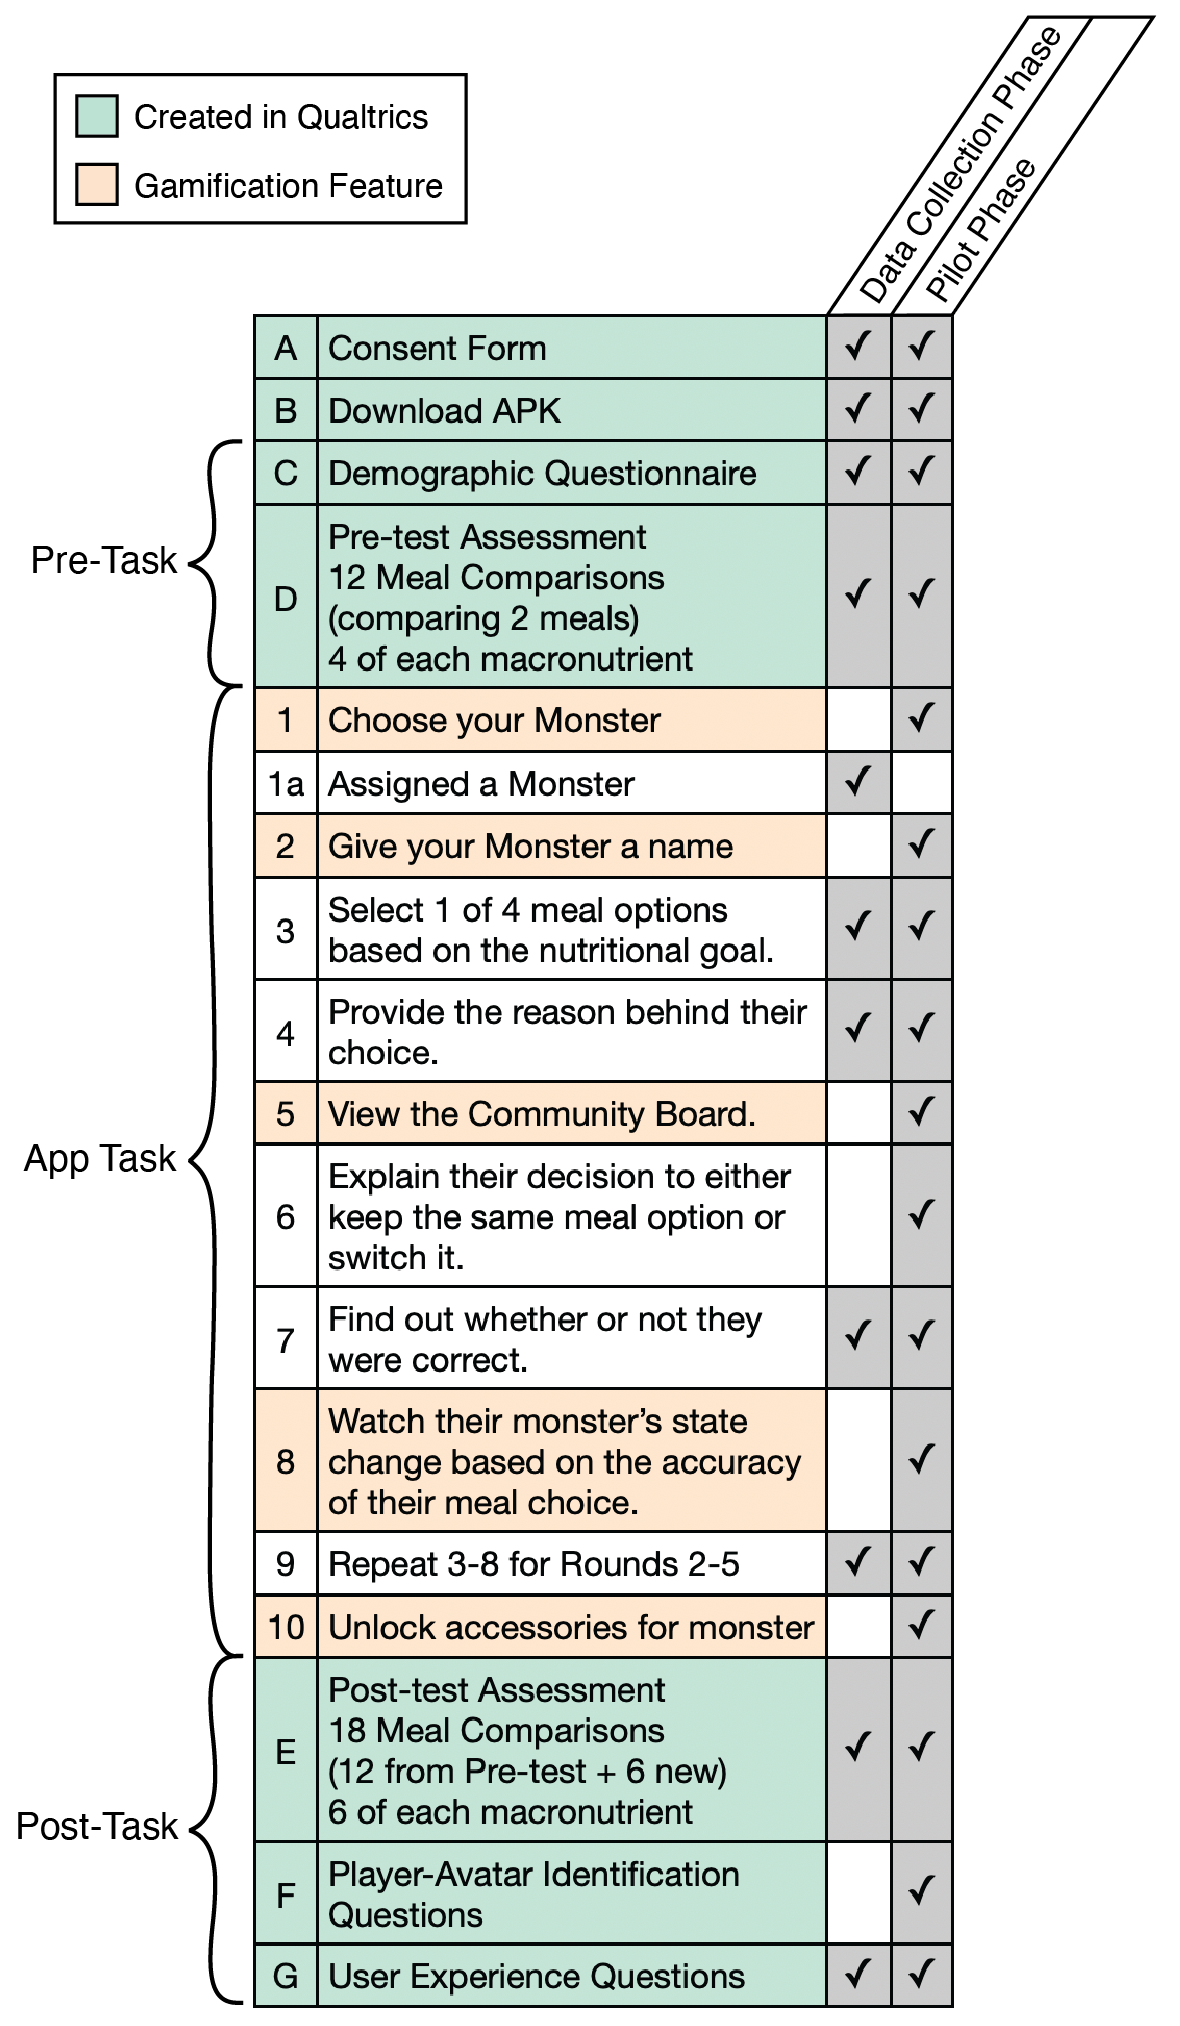
\includegraphics[width=\linewidth]{samples/images/figure-2-02.png}
\caption{Chart showing the steps of the study and the differences between the data collection phase and the experimental phase.}
\label{fig:phasechart}
\end{wrapfigure}

In this section, we outline the processes of preparing the tools we used in our study, including the survey elements of the pre-app task and post-app task, as well as the app itself.

\subsection{Development of the App}

The app was created using the visual programming interface, MIT App Inventor 2, version nb185a, and exported as a Android Package Kit using MIT App Inventor Code, version code36. An Android Package Kit (APK) is a file format used by Android to distribute and install apps.
%%Due to the 10MB APK limit in AI2, after we created the app, we had to export it as an .aia file, the native format for App Inventor apps. To build the APK, the .aia file was then imported into MIT App Inventor Code, version code36, which has a capacity for building APK files up to 50MB. 

The app was programmed to collect detailed logs of users' interactions (i.e., clicks, time-stamps) to assist in identifying user behavior and level of interaction. 
The app also randomized the meal choices within each round, as well as the order of the rounds themselves.



\subsection{Meal Photo Selection}
The app features 37 photographs of ``in-the-wild'' meals.
\textcolor{blue}{The images were gathered from a set used in one of the researchers prior crowdsourcing-in-nutrition~\cite{desai2019personal,mitchell2019wish} studies for which the expert nutritional assessment provided by a professional dietitian was available. HOW DO WE PHRASE THIS??}
We filtered the images based on their resolution quality and content clarity, so that users were able to easily identify the components of the meals.

In each round, users were presented with four ``in-the-wild'' meal photographs.
We created the rounds so that each round consisted of one best choice, one second best choice, and two less desirable choices, ranked as such by their macronutrient content assessment. 

%%-- filtering the ``in-the-wild'' meal photographs
%%-- nutrition experts helping us choose meals and or reasons (creating a ground truth)
  
%(MENTION THAT THE IMAGES ARE FROM MEALYZER AND THEN REFERENCE GLUCOGOAILIE OR GLUCORACLE STUDY -- so that we can say they are from our previous studies)


We tested the accuracy of the meal choice rankings by circulating all rounds to nutrition experts. 
We then adjusted the rounds as necessary to achieve above 50\% expert agreement for all rounds. 



\begin{figure}[h]
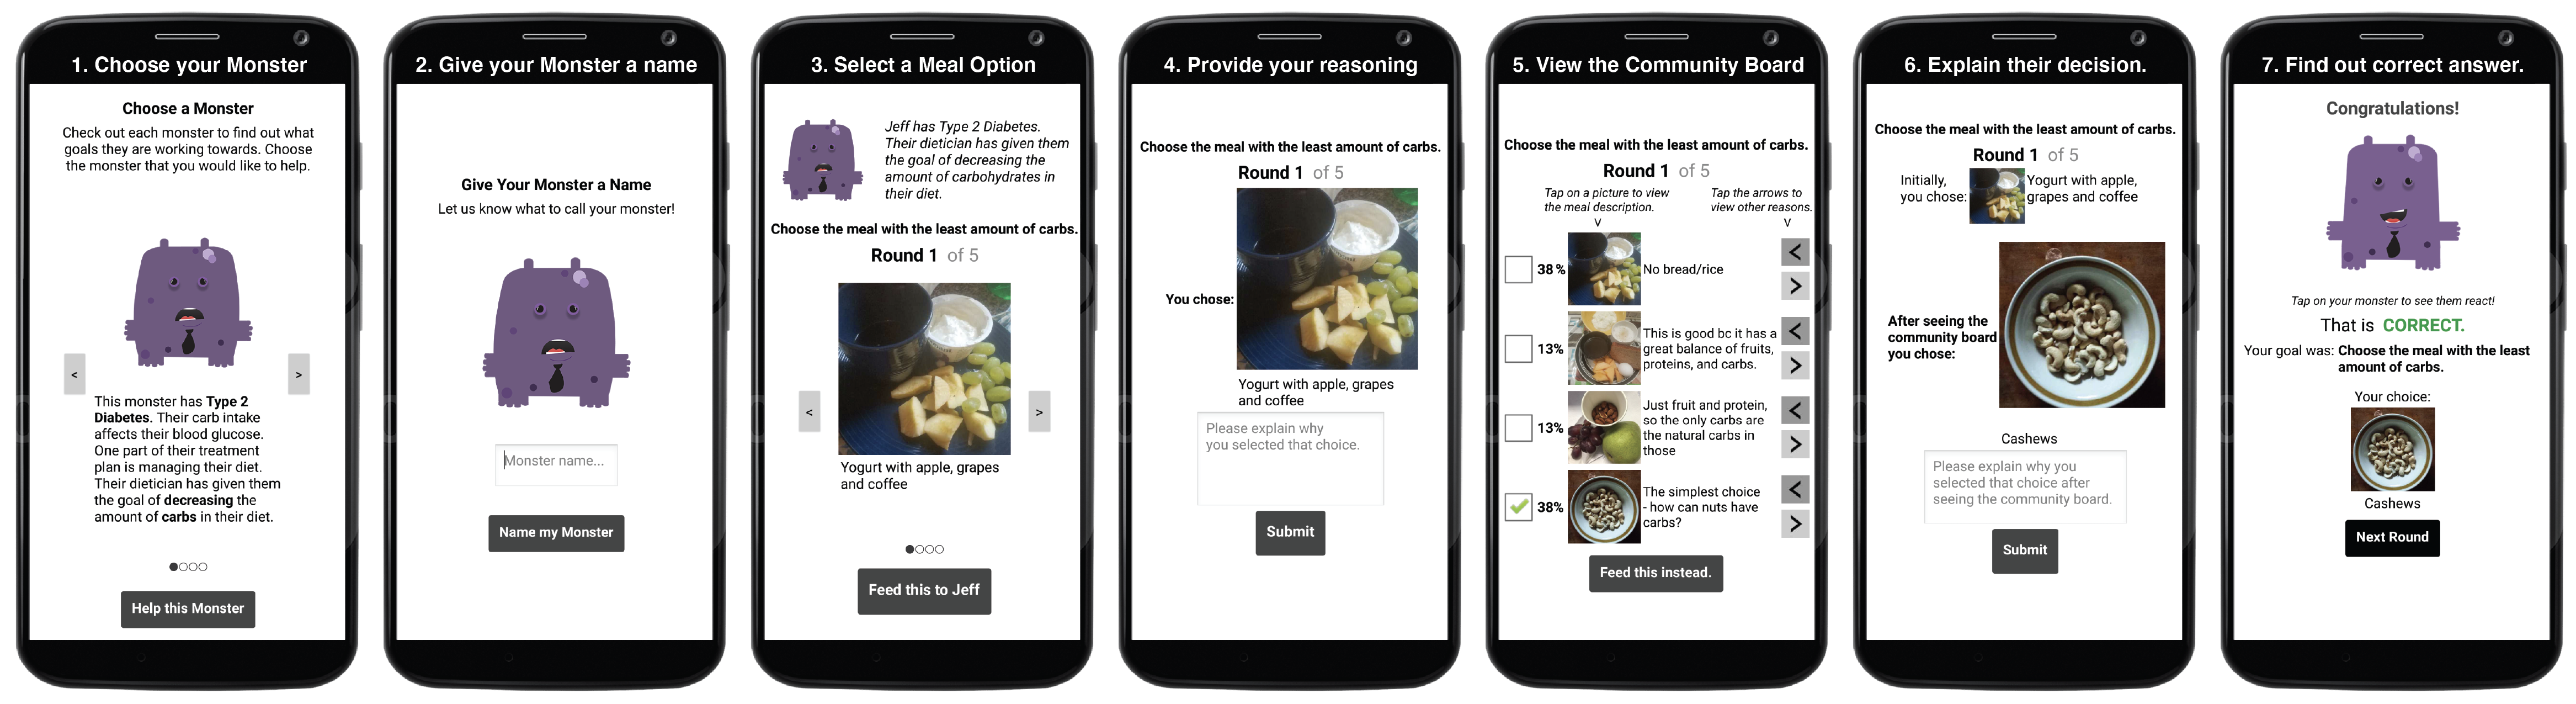
\includegraphics[width=\textwidth]{samples/images/figure-3.png}
\caption{Series of screenshots showing the main steps of the app.}
\label{fig:screenshots}
\end{figure}

%-- to refer to some figures as you explain the steps of the game
%-- game design choices
%-- why four meals per round than more
%-- connection to firebase


%The four stories were: 1) This monster has Type 2 Diabetes. Their carb intake affects their blood glucose. One part of their treatment plan is managing their diet. Their dietitian has given them the goal of decreasing the amount of carbs in their diet. 2) This monster is clinically overweight. They want to lose weight and become more healthy. One part of their plan is managing their diet.  Their dietitian has given them the goal of decreasing the fat content in their diet. 3) This monster has been training to run a marathon. Their big race is coming up. One part of their plan is managing their diet. Their dietitian has given them the goal of increasing the amount of carbs in their diet. and 4) This monster has Irritable Bowel Syndrome. Their daily life is greatly influenced by the way their digestive system behaves. One part of their treatment plan is managing their diet. Their dietitian has given them the goal of increasing the amount of fiber in their diet. 


\subsection{Gamification Features}
The Experimental Phase (EP) differed from the Data Collection Phase (DCP) with inclusion of Gamification Features (GF). 
%The GF occur throughout the game-play of the app. 
They can be seen within the context of the app and larger study flow in Figure~\ref{fig:phasechart}.

\subsubsection{GF1: The Ability for the User to Select and Name a Pet Monster Avatar}

There are four monsters in the app, each having their own brief background story as to why they are pursuing their nutritional goal. 
For example, one monster's story reads: \textit{This monster has Irritable Bowel Syndrome. Their daily life is greatly influenced by the way their digestive system behaves. One part of their treatment plan is managing their diet. Their dietitian has given them the goal of increasing the amount of fiber in their diet}. 

In the DCP, users were assigned to their monster and provided with its story and corresponding nutritional goal. 
In the EP, users could choose their own monster avatar with a corresponding health goal. After selecting one of the four monsters, users were asked to give their monster a name. 
This custom name was used throughout the rest of the game. 
Figure~\ref{fig:screenshots} shows screenshots of the app with the steps of the ``gameplay.'' 
Screen 1 is where users can tap through the carousel of monster choices to choose a monster to play with. Screen 2 shows how a user can give their monster avatar a custom name. The subsequent screens show an example of playing Round 1, where the custom name (e.g., ``Jeff'') can be seen implemented in the game.

\subsubsection{GF2: Viewing the Community Board of Crowdsourced Intelligence}

The inclusion of a community board (CB) allows users to view input from other users' to assist them in deciding which meal best fits the chosen nutritional goal. 
This CB displays both the percentage of users that selected each of the four meal options as well as three user-generated reasons as to why other users chose that meal option. The presented user-generated reasons were from those collected in the DCP. 
\textcolor{blue}{How should we explain that we also gathered "fake" reasons (with the google forms) so that every meal choice had three reasons (even if it showed 0\%)?}


%The inclusion of the community board will allow us to analyze how users decisions might be influenced by the (un)popular opinion and reasonings of other users. 
%We anticipate that in scenarios where the user is swayed by the community board and then shown to be incorrect, we will see a reluctancy in future rounds to trust the opinions of others over their own instincts. 
%However, this will most likely change when the community board helps the user find the correct answer, in which case we anticipate that it will be common to see the user trusting the opinions of others in the future.
  
\subsubsection{GF3: Monster State Change and Accessory Unlocking in Reaction to Meal Choice Accuracy}
%These gamification features provide a lightweight environment for users to gain exposure and knowledge about nutrition components of different meals.

\begin{wrapfigure}{l}{0.5\textwidth}
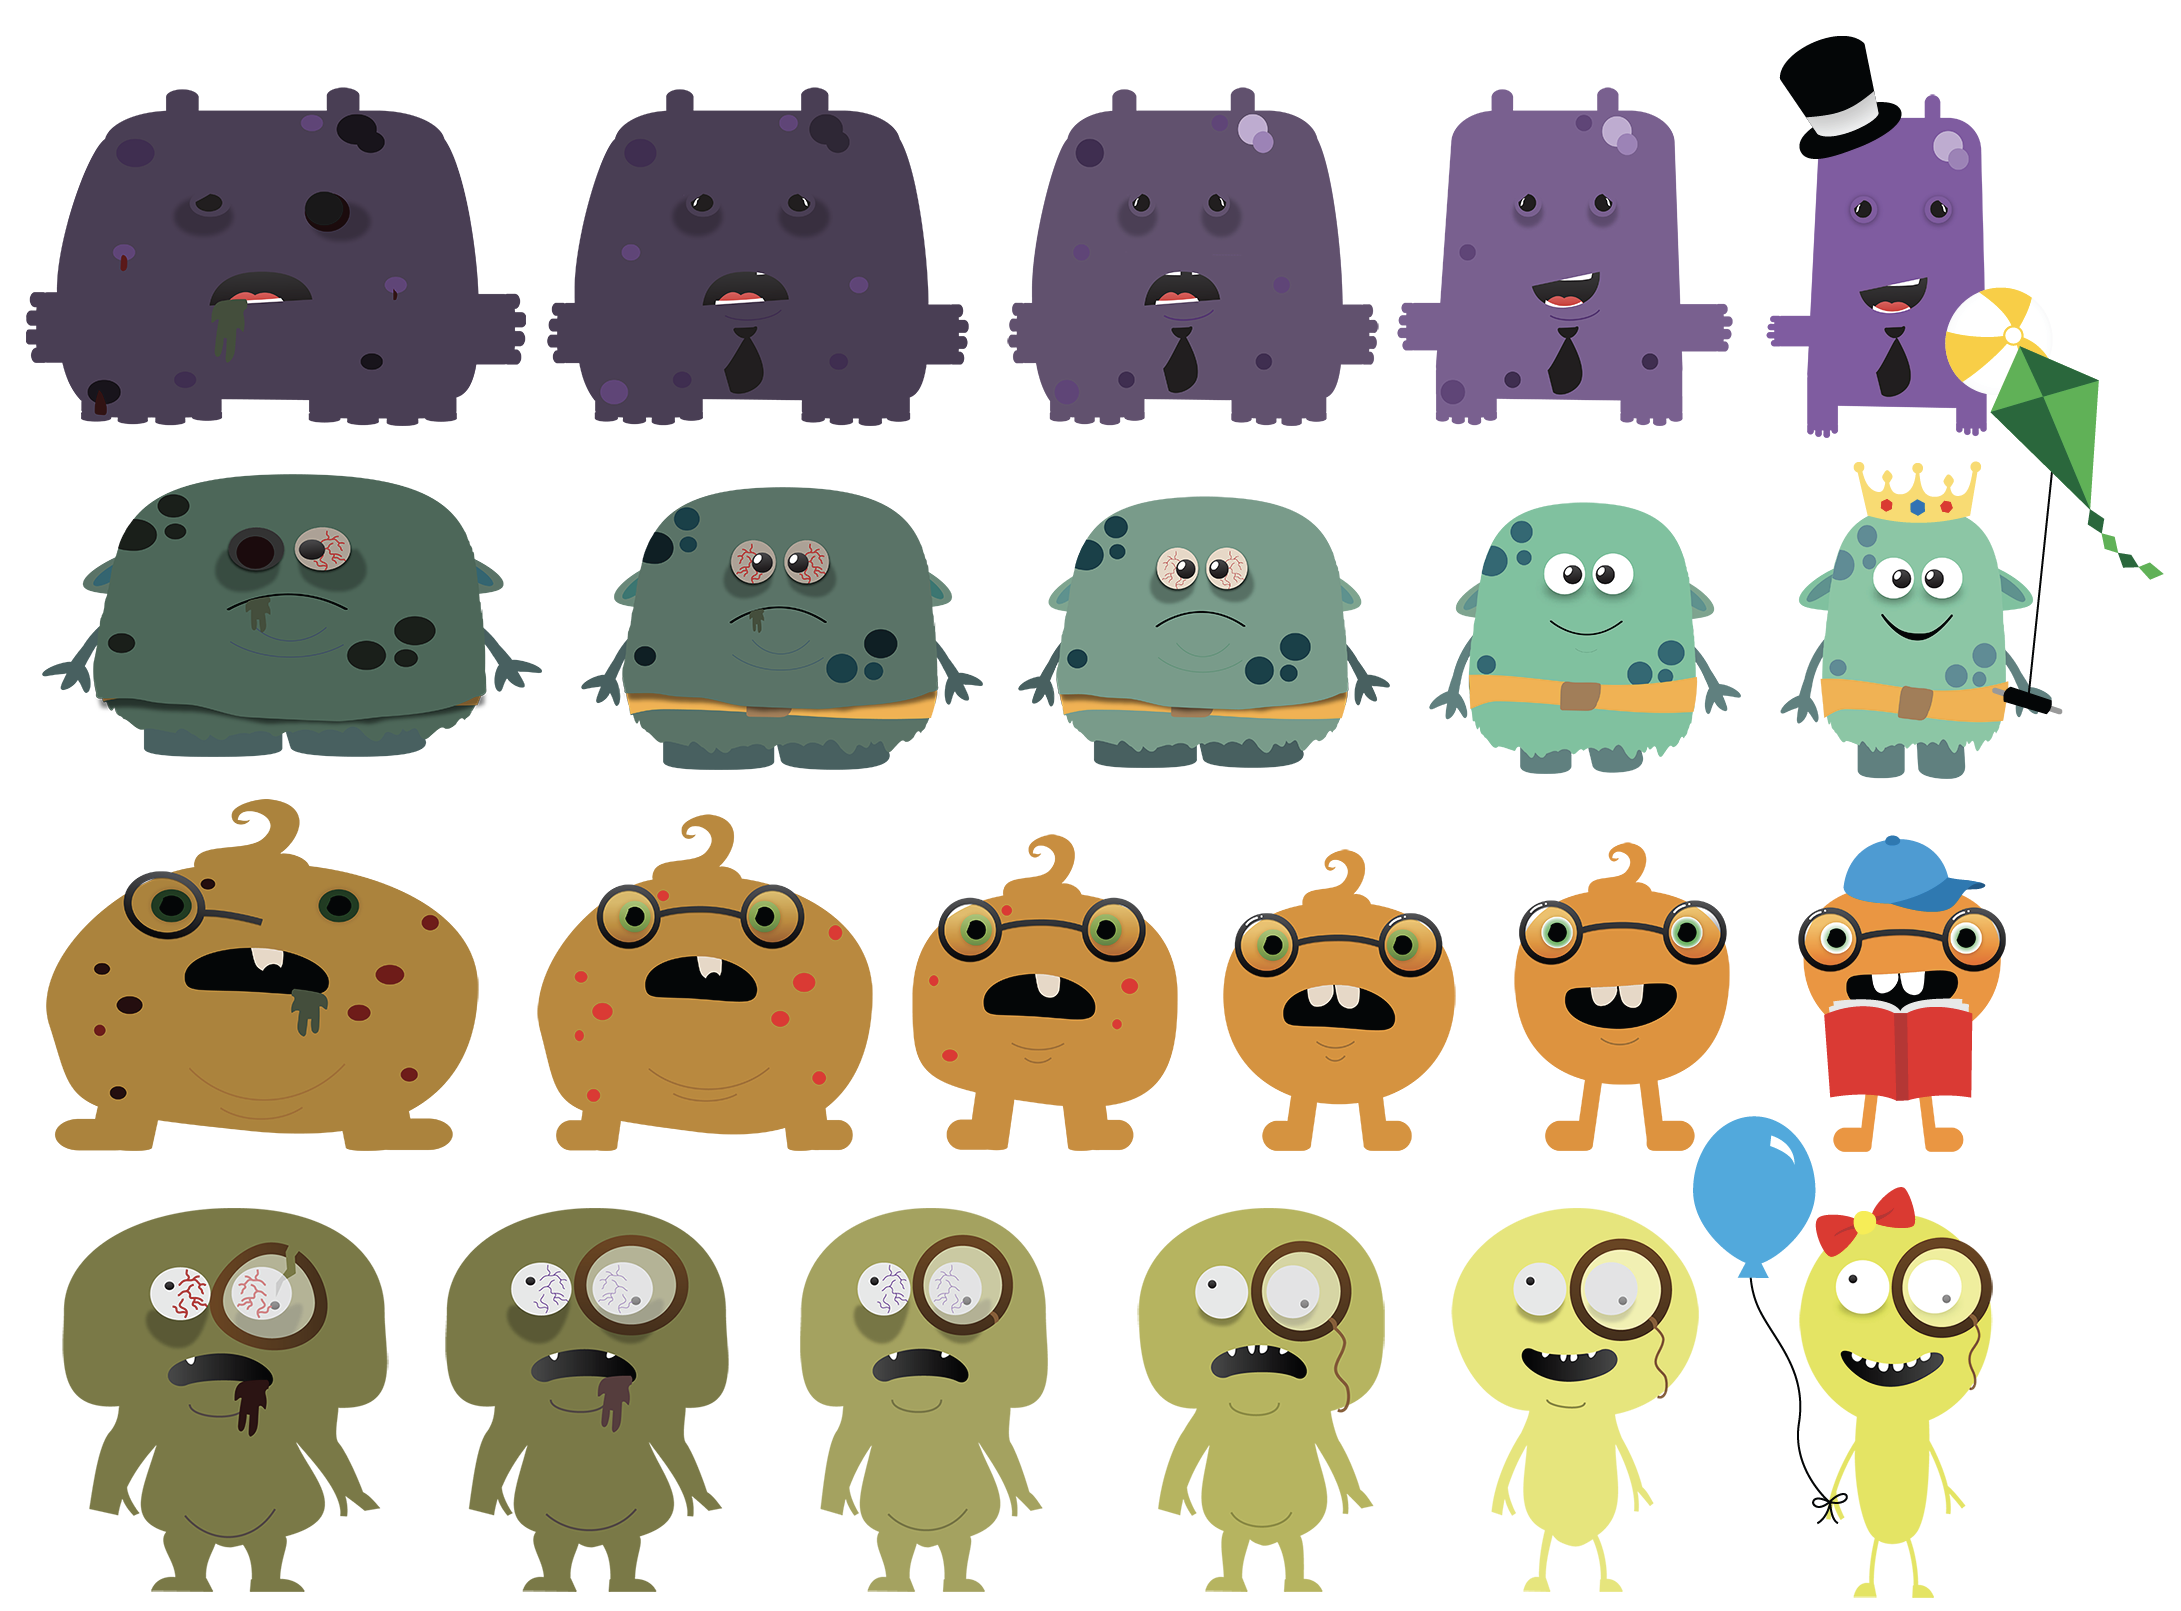
\includegraphics[width=\linewidth]{samples/images/figure-5.png}
\caption{Sample of various monster condition stages and available accessories.}
\label{fig:monster-stages}
\end{wrapfigure}
 
Once the user has viewed the CB and submitted their final meal choice, they will be able to watch their pet monster avatar react to the meal they have chosen to feed them. 
If the monster is fed the best choice meal for their nutritional goal, the user will see their monster avatar's physical state improve in a short animated morph.
If the user feeds their pet monster either the worst meal option, or the second to worst, they will see their pet monster's physical state degrade in the animated morph. 
If the monster is given the second best meal option, their condition neither improves nor worsens. 
%This visual feedback allows the user to see the impact of their choices for their pet monster, as well as motivate them to provide the best options in the future.
This game component also gave users the chance to earn and choose accessories for their pet monster. 
If within the five rounds of ``gameplay'' a user answers four or more questions with the best meal option, the user unlocked the accessories screen, where they were able to choose one of four accessories to award their pet monster. 
Given the five rounds, users could win up to two accessories.







Within the app, in each round, when the four images of meal choices were shown, each was accompanied by a brief description of its contents. 
Users were asked to select the meal option that they believed best fit their monster's nutritional goal. 
The app also prompted users to explain their reasoning for their meal choice.
After submitting their reason, users were told whether or not they selected the best choice and shown the correct answer.
This process of choosing a meal option, providing the reason why, and viewing the result was repeated for each of the five rounds.




\subsection{Development of pre-test and post-test }

The consent form, demographic questionnaire, pre-test assessment, post-test assessment, player-avatar identification questions, and the user experience questions were all created using the online survey platform, Qualtrics.

This is where we will reference Marissa's paper~\cite{burgermaster2017role} a lot -- this was our inspiration (her paper is mentioned in the Observational Learning subsection in the background section). 

+ Elliot's paper~\cite{mitchell2019wish} about carb choices -- we need to reference that too

``Learning outcomes that are seen as relevant to the effectiveness of DGBL are 1) increased interest in the subject matter, 2) improvement in objective performance (e.g., in a test), and 3) transfer, referring to the player's ability to apply acquired knowledge or skills to real-world situations.'' -- referenced from ``Towards a conceptual framework for assessing the effectiveness of digital game-based learning''~\cite{all2015towards}
--- this could be a good rationale for our decision in choosing the recall items (relates to 2) objective performance) and transfer items (relates to 3) transfer). What do you guys think?

We created the pre- and post-task surveys in the online survey platform, Qualtrics.

There were two pre-task surveys, a demographic questionnaire, and a pre-test nutritional assessment.
In the demographic questionnaire, users were asked basic demographic questions and questions about their prior experiences with nutritional knowledge and health related apps. The pre-test nutritional assessment consisted of 12 questions in which users were tasked with identifying which of two meal options better fit a given macronutrient content goal (e.g., which meal photograph is higher in carbohydrates). 
In these 12 questions, the participants did not receive feedback on the accuracy of their responses. 
The 12 questions were made up of 4 questions for each macronutrient (carbs, fat, fiber). 

The post-task consisted of three surveys: the post-test assessment, the player-avatar-identification (PAID) 
The post-test assessment was similar to the pre-task survey in that it was also made up of two parts: 18 questions where the user was asked to identify which of two meal options better fit a given macronutrient content goal, and follow-up questions related to their experience in the study. 
The 18 meal identification questions consisted of 6 questions for each of the three macronutrients, with 4 questions containing meals repeated from the pre-task survey, and 2 questions containing meals that were new to the user. 
\vspace{-5pt}
\section{Monster Munch Pilot Evaluation Study}

The pilot evaluation study for the Monster Munch app was conducted with participants recruited via 
Amazon Mechanical Turk (AMT) and social media sites. The goals of the evaluation study were to (1) to assess users general perceptions using a lightweight app for engaging with nutrition and (2) understand how the different gamification mechanisms built into the app (avatars and crowdsourced community board) shape users preferences and experience with the app. The pilot study followed the procedure outlines below and summarized in Figure~\ref{fig:studyflow}. 


\begin{figure}[h]
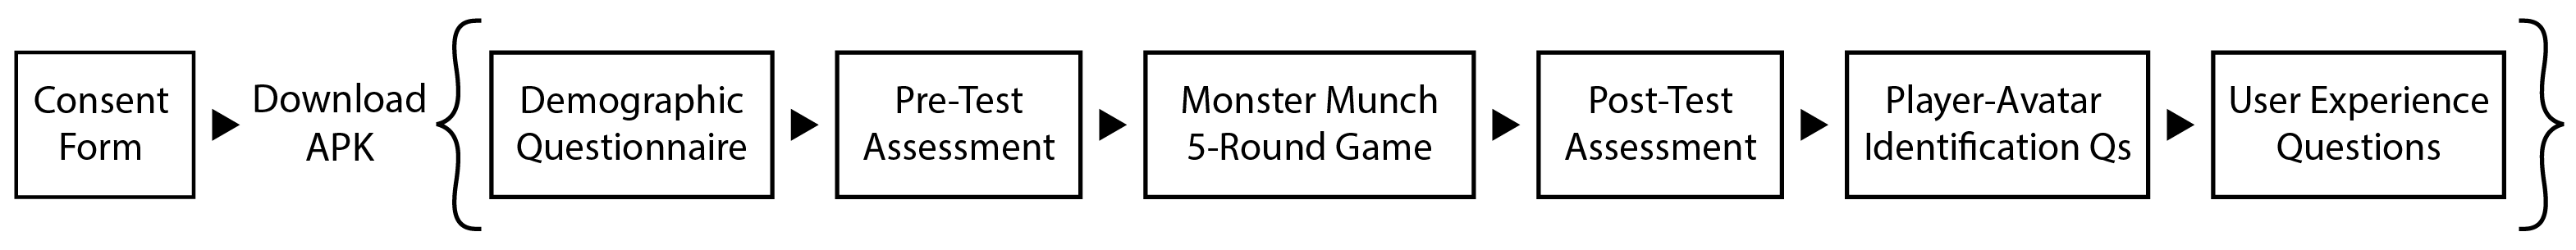
\includegraphics[width=\textwidth]{samples/images/figure-1.png}
\caption{Study flow for participants in the Monster Munch pilot study. Study sections indicated inside the curly braces were completed within the mobile app. }
\label{fig:studyflow}
\end{figure}

\vspace{-5pt}
\subsection{Participant Recruitment}
Participants were recruited from AMT and social media sites (Facebook and Instagram). Users were screened with the following inclusion criteria: 1) own an Android mobile device, 2) above 18 years of age. After accepting the terms of the study found in the consent form, participants  downloaded an APK file and installed the Monster Munch app. Within the app they completed a pre-test evaluation, completed the nutrition task with monsters, and completed a post-test assessment and surveys. Only participants who completed the pre-test evaluation, the Monster Munch app, and post-test evaluation were considered in subsequent analysis. 


\vspace{-5pt}
\subsection{Monster Munch App Activities}

In the Monster Munch app, users could view each of the four pet monster avatars and their nutritional goals before selecting one to proceed with and ``help'' during the game. Users also had the opportunity to give their monster a custom name before completing the task and helping feed their monster.

In the core monster feeding task, users selected meals to feed their chosen monster for five rounds. Each round of meal selection consisted of five steps. 
At the first stage of each round, the user was presented with  four options of ``in-the-wild'' meal photographs, accompanied with brief descriptions of the contents of each meal that they could review to decide what to feed their monster. Second, users were asked to select the meal that they believed best fit their monster’s nutritional goal and provide a short text-based description of why they selected that particular option. Third, users viewed the crowdsourced CB where they could consider which meal other members of the community chose to feed their monster. Users could view the percent of users that selected each meal and their reasoning for doing so (these percents and rationales were sourced from the implementation pilot described above). Fourth, armed with this new information, users had the option to keep their original meal selection, or switch to another meal option. Again, users were asked to provide a short description to rationalize their final meal selection after viewing the input from the CB.
Finally, after they submitted their reasoning, the app told the user whether the meal option they selected was (in)correct, and which meal option was the best choice. The appearance of the monster avatar also changed in response to the user's performance, becoming ``healthier'' if the user selected the correct meal, and ``less healthy'' if the user selected the incorrect meal. 

Users repeated these steps for each five meal selection rounds with their same  monster avatar, helping them work towards their monster's nutritional goal.
\vspace{-5pt}
\subsection{Data Analysis and Measures of Interest}
Participants' survey responses were collected via Qualtrics and their engagement with the app  collected via the Google Cloud computing platform Firebase and extracted with Python 2.7 (script available on Github at \url{provide_later}). Users' data from Qualtrics and Firebase were merged together for processing, and 
%\url{https://github.com/mlhwang/m4m}
Statistical Package for the Social Sciences (SPSS version 27) was used to analyze the data. For all analysis the alpha significance threshold was set at 0.05.  

\subsubsection{Player Avatar Identification}
Users' engagement with the gamified avatar component of the task was assessed with four Player Avatar Identification (PAID) questions asked in the post-task survey (adapted from~\cite{li2013player}). Users indicated their agreement to the following four statements on a 7-point likert scale (with the option to select ``Not Applicable''): 
\begin{enumerate}
    \item ``When my monster’s condition worsened, I felt angry/sad.''
    \item ``When my monster achieved their goals, I felt happy.''
    \item ``My monster reflects who I am.''
    \item ``My monster influences the way I feel about myself.'' 
\end{enumerate}
A ``PAID score'' was calculated for each user by summing their responses to each question. Higher PAID scores indexed stronger player-avatar identification.

\subsubsection{Community Board Agreement}

The community board (CB), was created through the Data Collection Phase. The two CB related questions during the post-app task included: 
\begin{enumerate}
    \item ``Did the community board influence your final meal choice?'' 
    \item ``How often did you agree with the rest of the community?'
\end{enumerate}

Users responded on a scale of `Always;' `More than half of the time;' `About half of the time;' `Less than half of the time;' `Never;' and `I did not look at the community board.' 

\subsubsection{Macronutrient Knowledge Assessment}

Macronutrient knowledge was evaluated before and after the Monster Munch app activities. Users completed a 12-question pre-test for which a percentage correct was calculated to establish a baseline for nutritional knowledge. After the Monster Munch app, users completed an 18-question post-test, that contained the 12-questions asked in the baseline evaluation and six additional questions. Performance on the 12 repeated questions was used to assess recall of nutrition knowledge, and performance on the six new questions was used to assess transfer of nutrition knowledge in comparison to the baseline evaluation. 
\vspace{-5pt}
\subsection{Research Questions}
In the next section we discuss the results from this pilot study using Monster Munch. In particular this pilot evaluation was centered around understanding the following questions:
\begin{enumerate}
    \item Does playing Monster Munch influence users' confidence of their ability to estimate macronutrient content of ``in-the-wild'' meal photographs (a proxy for nutritional engagement)?
    \item Does the inclusion of gamification mechanisms (pet monster avatars and crowdsourced community board) influence enjoyment/engagement of the Monster Munch app?
    \item Do gamification mechanisms have an effect on nutritional learning (a proxy for nutritional engagement)?
\end{enumerate}

% The hypotheses are:
% \begin{itemize}
%     \item \textbf{H1}: User's will report higher enjoyment and show greater engagement with the Monster Munch app after the inclusion of Gamification Mechanisms. 
%     \item \textbf{H2}: Monster Munch (a mobile app for nutritional engagement) will help users become more confident in their ability to assess macronutrient content of ``in-the-wild'' meal photographs pre- to post-test.
%     \item \textbf{H3}: Users who chose pet avatars with a health goal that is personally meaningful in Monster Munch are more likely to perform better (i.e., identify the right meal photographs for a specific nutritional goal) pre- to post-test.

% \end{itemize}

%\subsubsection{Data Collection Phase (DCP)} The three primary goals of the DCP were to 1) collect user-generated responses to use within the `Monster Munch' community board in the EP, 2) provide initial insights on the prior knowledge and nutritional literacy of lay users, and 3) assess the user experience and data collection methods of the app. To accomplish these goals, users in the DCP completed both a pre- and post-task, and a simplified version of the app, without the gamification mechanisms (GM) used in the EP. In the DCP, every user was assigned one of the four pet monster avatars. The user was introduced to their monster avatar and its nutritional goal before proceeding to the five rounds. 

%There will be three steps for the user in each of the five rounds. First, the user was presented with the four options of ``in-the-wild'' meal choices, where they selected the meal that they believed best fit their monster's nutritional goal. Next, the user was asked to provide a short description of why they selected that particular option. Finally, after the user submitted their reasoning, the app revealed whether the meal option they selected was correct, and if they were incorrect, which meal option was the best choice. Each user repeated these three steps for all five rounds with the same pet monster avatar and its nutritional goal. 

%The app in the EP differs from the DCP with the addition of the GMs.

%%% Is this sort of thing needed for CHI?%%%
%\subsection{Analysis}
%We will use a combination of qualitative and quantitative methods to analyze the data collected during the proposed study. For the quantitative measures collected during the study (results of their scores on different questionnaires and accuracy of their nutritional assessment), we will use appropriate statistical tests to examine the differences in means for the measures of interest.
\vspace{-5pt}
\section{Results}

In the results, we focus around three key themes: (1) users' general experiences with the Monster Munch app; (2) the importance of gamification mechanisms in shaping users' experiences with the app; and (3) the role of gamification mechanisms in facilitating nutrition recall, reflection, and learning. (\textit{All tables for all analyses are provided in the supplementary material for full description and inspection}.)




\vspace{-5pt}
\subsection{Participant Background}
Sixty eight participants completed the pilot study. Participants' ages ranged from 18 to 65, with most participants falling into the \textcolor{red}{XX-YY group}. Participants were evenly split across gender (44\% female) and education level (50\% above high school/GED or equivalent). Most participants reported not working professionally in nutrition (75\%) and having no prior experiences with using health applications (60\%). In choosing which monster to select, participants preferences were relatively evenly distributed across each of the four monster options: Monster 1 for Type 2 Diabetes (27.9\%), Monster 2 for Weightloss (27.9\%), Monster 3 for Running a marathon (27.9\%), and Monster 4 for Irritable Bowel Syndrome (16.2\%). \textcolor{red}{Should we also include the corresponding nutrients/nutritional goals?}
\vspace{-5pt}
\subsection{General Experiences with Monster Munch}

Overall, users liked playing the game and found it a useful tool for reflecting on nutrition. One participant reflected this sentiment by commenting: \textit{``This was fun and I think someone can learn a lot about nutrition through trial and error''} (ID-072424). Additionally, we discovered that users self-reported confidence in assessing macronutrients from meal photographs statistically significantly improved after a single interaction with the app (Paired T-Test, pre-post scores \textit{t}=-.3.484, \textit{p}=.001, \textcolor{red}{ES = ).} %We subtracted the post-app contfidence scores from that of the pre-app yielding in a negative mean 
\vspace{-5pt}
\subsection{Gamification and the Monster Munch Experience}

Next, we sought to understand how the gamification mechanisms of the app contributed to users' experience and enjoyment of the app. 

\vspace{-5pt}
\subsubsection {Avatar and User Experience}
We were interested in how users interacted with avatars, and how that in turn shaped their experiences with Monster Munch. Users reported their primary reasons for selecting the avatar to be: because they or someone they knew was working on the same goal, because they wanted to learn more about the health goal, and because they liked the appearance of the monster.

We assessed the degree users identified with their avatar through a series of questions calculated into a composite ``PAID score'' that measured users' affinity with their avatar (refer to section 4.3.1). 
User's PAID score did not vary significantly across any demographic categories other than education; with regards to education users who reported having a high school education or less identified significantly more with their avatars (Independent T-Test; \textit{p}=0.003, Cohen's \textit{d} ES=0.77). 
Then, we examined  how users' affinity towards their avatars related to their enjoyment of the game. We found stronger identification with the avatar significantly predicted app enjoyment \textcolor{red}{(B=0.11, \textit{p}<0.001),} app recommendation (B=0.92, \textit{p}< 0.001), and app rating (B=0.22, \textit{p}<0.001).
Lower educational background was associated with higher app enjoyment (\textit{p}=0.021, Cohen's \textit{d} ES=0.59). However, education did not appear to significantly explain \textcolor{red}{any of these effects --do you mean any of the rest of the app related effects? ... I'm confused as to the why this sentence is included..?}. 
Further, avatar identification was not significantly related with users' overall meal choice performance within the app, even after controlling for prior nutritional knowledge and educational background (\textit{p}=0.079). 

\vspace{-5pt}
\subsubsection {Community Board and User Experience}
We were also interested in how the second gamification mechanism embedded into the app design, the crowdsourced community board, might shape user's experience.
Broadly, user experience with the community board did not vary significantly across any demographic categories. However, we observed that user's self-reported influence by the community board's information significantly predicted their enjoyment of the app \textcolor{red}{(B=0.267, \textit{p}=0.001),} how they rated the app \textcolor{red}{(B=0.469, \textit{p}=0.011)}, and willingness to recommend the app to others \textcolor{red}{(B=0.281, \textit{p}<0.001)}. 

%{PROBABLY IN DICUSSSION?? Together these findings highlight the importance of users engagement with gamification components to their overall experience using and enjoying the app. }

\vspace{-5pt}
\subsection{Avatar Identification and  Nutrition Recall}

Although nutritional literacy or learning was not a core focus on this feasibility-oriented pilot study, the inclusion of a baseline and post-task nutritional assessment allowed us to investigate preliminary measurements to see if gamification in Monster Munch might relate to improved recollection of nutritional information and indicate that the app has the potential to become a future learning tool. We compared pre-task nutrition macronutrient assessment scores to performance on the same questions post-task and found significant improvement in the post-task evaluation after completing the Monster Munch app (Paired T-Test; \textit{t}=-2.392, \textit{p}=.020).

%We then looked to see how the gamification components might relate to performance on the post-test. 
We found that lower player-avatar identification marginally predicted greater recall of nutrition information, even after controlling for baseline nutrition knowledge, educational background, and Monster Munch task performance (\textit{B}= -0.009, \textit{p}= 0.051). Additionally, while both pre- and post-score nutritional assessment  predicted recall, there was no significant interaction between individuals pre-score assessment and avatar identification (\textit{p}=0.32). 
%Through these findings avatar identification emerges as an important possible predictor of nutritional knowledge recall. 

Looking at other gamification elements, users who indicate greater use of the community board performed significantly worse on cursory measures for recall after controlling for prior nutritional knowledge (\textit{B}= -0.036 , \textit{p}=0.006).


REMMEBER THAT IN PRE AND POST TEST THEY HAD TO CHOOSE FROM TWO MEALS WHICH HAS A BETTER CHANCE OF GETTING IT RIGHT THEN CHOOSING FROM FOUR MEALS





\vspace{-5pt}
\subsection{User Experience Open-Ended Feedback}
At the end of the survey, we asked participants to leave any comments or feedback about the overall study. 
Some of them specifically mentioned their experience using the app: \textit{``I think someone can learn a lot about nutrition through trial and error via this [app] instead of using their own body as an experiment''}(ID-??????)
\textcolor{blue}{We already included this quote in a prior section (5.2) line 11}
The average time all the users spent (measured in seconds) in the app was \textcolor{red}{(\textit{M}(68)= , \textit{SD}= --UPDATE THESE \#)}. 
Regarding time spent with the app, one user wanted to experience the app for an extended period and expressed there may be potential with a better narrative: \textit{``My investment might have been higher if it was longer and there was more [continuity]...Overall great [app] with great potential. Perhaps if the narrative and continuity is further developed''} (ID-100243). %Unsurprisingly, among the 68 participants only a handful left such feedback for the research team, as it was an optional question at the very end of the entirety of the study. 


% One user from each phase mentioned wanting to have the recipes of the meal photographs that were shown to them. 
\section{Discussion}
SOME RANDOM TEXT INCLUDED HERE.

\subsection{Learning}

\subsection{Player Avatar Identificaiton}
Meaning of high player identification scores but low learning scores. What can we make of that?

\subsection{Crowdsourced Intelligence}

Community board from Phase 1 but do not forget now we have an even more massive community board from Phase 2. 

\subsection{Limitations}

Limitations of this research study in this particular scope is discussed in the following sections. 

\subsubsection{Limitations with the Gamification Features}

For the "unlock accessory" feature, players were not made aware accessories were available to ``upgrade'' one's monster avatar if four rounds and five rounds worth of meals were correctly fed to the avatar. 

There was also no final winning or losing status mentioned to the players. We probably should have made it clear that there were unlocking accessories avail and once you reach that level you have actually ``won'' the game (though we are not calling this officially a game). 



\subsubsection{The Quality of the Users' Responses -- threats to validity?}
How much can we trust the Turkers that they indeed only had up to a high school degree when we were doing purposeful sampling. 

How much can we guarantee that the post-test responses were not influenced by fatigue. (Maybe this is a good place to quickly mention the average duration people took to complete the entire study? -- first mention this in the Evaluation section when maybe talking about Participants)


\subsubsection{Determining the Gold Standard for ``in-the-wild'' Meal Photographs}
First of all, we involved quite a number of people to achieve this. But also the meal photographs are from our previous studies~\cite{} -- keep it anonymized-- and that means most meals are from a particular geographical population (Washington Heights). In creating a true ``crowdsourced intelligence'' driven community board we would have to do a much more comprehensive collection of meal photographs. Maybe using soical media sites like IG and TikTok might help?


Taken from \cite{cuthbert2019effects}:
``Secondly, this study had a small number of participants
which made the statistics very vulnerable to type II errors.
We tried to deal with this limitation by reporting effect sizes,
descriptive statistics, and all the p values, avoiding the typical
practice of sharing only statistically significant results.''

\subsection{Future Work}

How do we get to a truly crowdsourced community board that really represents all people and all types of food? Is that even possible? Could there be one place, one repository for this, or should there not be just one repository? How can we do this more at scale?


\vspace{-5pt}
\section{Conclusion}
We piloted Monster Munch as a feasibility-focused study to investigate two major gamification mechanisms: player avatar identification and crowdsourced community board. Though avatars appear frequently as a game mechanic in games and gamified apps, they are not often paired with crowdsourced social features and investigated in conjunction with learning. From our pilot study, we witnessed that these mechanisms were not only welcomed by the users, but also they encouraged them to engage with macronutrient nutrition topics based on crowdsourced meal photographs. Though the avatar bond from the user was negatively associated with nutrition learning, the pilot highlights these mechanisms as effective tools to further discuss lightweight approaches for nutritional engagement. Future studies should investigate the right combination of gamification mechanisms that can promote nutritional engagement to improve nutritional literacy.

All APKs and relevant data pre-processing and data extraction scripts are available on our Github for the HCI community (anonymous link here). 

%%
%% The acknowledgments section is defined using the "acks" environment
%% (and NOT an unnumbered section). This ensures the proper
%% identification of the section in the article metadata, and the
%% consistent spelling of the heading.
\begin{acks}
This is partly funded through ABC University's hungry hungry monster grant.
\end{acks}


%%
%% The next two lines define the bibliography style to be used, and
%% the bibliography file.
\bibliographystyle{ACM-Reference-Format}
\bibliography{acmart}
%sample-base

%%
%% If your work has an appendix, this is the place to put it.
\appendix


%\section{Supplementary Tables}

\subsection{Experience with Monster Munch}

%%%%%%%%% CONFIDENCE %%%%%%%%%%%%
\begin{table}[!h]
  \caption{Macronutrient Confidence. Paired samples t-test of self-reported confidence in identifying macronutrients (i.e., fat, carbohydrates, fiber) from meal photographs pre and post using the app. \textsuperscript{**}$p<.01$, 
  \textsuperscript{*}$p<.05$} 
  %\textsuperscript{*}$p<.1$}
  \label{tab:confidence}
  \begin{tabular}{clrccc}
    \toprule
    Pair&N&Mean&Std. Dev&t&Sig. (2-sided)\\
    \midrule                                  
    Confidence Pre to Post  &67 &-6.075  &14.274 &-3.484   &0.001*\\
    \bottomrule
% \addlinespace[1ex]
\end{tabular}
%   \vspace*{-\baselineskip}
\end{table}


\subsection{Gamification Experience}

\subsubsection{Experience with Avatars}
Player Avatar Identification (PAID) is the independent variable. B: Unstandardized B; SE: Coefficients Standard Error; Beta: Standardized Coefficients Beta.

\textcolor{
\begin{table}[!h]
  \caption{Player Avatar Identification by Education Group. Independent t-test comparing PAID scored by Education Group (high school and below, high school and above). 
  \textsuperscript{**}$p<.01$, 
  \textsuperscript{*}$p<.05$} 
  %\textsuperscript{*}$p<.1$}
  \label{tab:confidence}
  \begin{tabular}{clrccc}
    \toprule
    Pair&N&Mean&Std. Dev&t&Sig. (2-sided)\\
    \midrule                                  
    Confidence Pre to Post  &67 &-6.075  &14.274 &-3.484   &0.001*\\
    \bottomrule
% \addlinespace[1ex]
\end{tabular}
%   \vspace*{-\baselineskip}
\end{table}
}

% PAID SCORE  FOR GAME ENJOYMENT AND EXPERIENCE %%%

\begin{table}
  \caption{Avatar Identification and App Enjoyment. Simple linear regression with app enjoyment as the dependent variable; PAID score as the independent variable.
  \textsuperscript{**}$p<.01$, 
  \textsuperscript{*}$p<.05$} 
  \label{tab:appenjoy}
  \begin{tabular}{cccccccccc}
    \toprule
    &B&SE&Beta&\textit{t}&\textit{p}&$R^{2}$&Adj. $R^{2}$&\textit{F}&\textit{p}\\ % $\eta_{\text{p}}^{2}$$
    \midrule                                  
     Model (constant)& &  & &  & &.266&.255&23.598&0.000\\
     PAID&.110 &.023  &.516 &4.858   &0.000**&&&&\\
    \bottomrule
% \addlinespace[1ex]
 \end{tabular}
\end{table}

\begin{table}
  \caption{Avatar Identification and App Recommendation. Simple linear regression with app recommendation as the dependent variable; PAID score as the independent variable.
  \textsuperscript{**}$p<.01$, 
  \textsuperscript{*}$p<.05$} 
  \label{tab:apprec}
 \begin{tabular}{cccccccccc}
    \toprule
    &B&SE&Beta&\textit{t}&\textit{p}&$R^{2}$&Adj. $R^{2}$&\textit{F}&\textit{p}\\ % $\eta_{\text{p}}^{2}$$
    \midrule                                  
     Model (constant)& &  & &  & &.212&.199&17.444&0.000\\
     PAID&.092 &.022  &.460 &4.177   &0.000**&&&&\\
    \bottomrule
% \addlinespace[1ex]
 \end{tabular}
\end{table}

\begin{table}
  \caption{Avatar Identification and App Rating. Simple linear regression with app rating as the dependent variable; PAID score as the independent variable.
  \textsuperscript{**}$p<.01$, 
  \textsuperscript{*}$p<.05$} 
  \label{tab:appenjoy}
 \begin{tabular}{cccccccccc}
    \toprule
    &B&SE&Beta&\textit{t}&\textit{p}&$R^{2}$&Adj. $R^{2}$&\textit{F}&\textit{p}\\ % $\eta_{\text{p}}^{2}$$
    \midrule                                  
     Model (constant)& &  & &  & &.225&.213&18.545&0.000\\
     PAID&.220 &.051  &.474 &4.306   &0.000**&&&&\\
    \bottomrule
% \addlinespace[1ex]
 \end{tabular}
%   \vspace*{-\baselineskip}
\end{table}

\textcolor{
\begin{table}
  \caption{Avatar Identification and App Performance. Simple linear regression with performance on the Monster Munch task as the dependent variable; PAID score as the independent variable.
  \textsuperscript{**}$p<.01$, 
  \textsuperscript{*}$p<.05$} 
  \label{tab:apprec}
 \begin{tabular}{cccccccccc}
    \toprule
    &B&SE&Beta&\textit{t}&\textit{p}&$R^{2}$&Adj. $R^{2}$&\textit{F}&\textit{p}\\ % $\eta_{\text{p}}^{2}$$
    \midrule                                  
     Model (constant)& &  & &  & &.212&.199&17.444&0.000\\
     PAID&.092 &.022  &.460 &4.177   &0.000**&&&&\\
    \bottomrule
% \addlinespace[1ex]
 \end{tabular}
\end{table}
}

\subsubsection{Experience with Community Board}
Community Board Influence (CBI). B: Unstandardized B; SE: Coefficients Standard Error; Beta: Standardized 
  \textsuperscript{**}$p<.01$, 
  \textsuperscript{*}$p<.05$} 
  
%%%%% SLR: COMMUNITY BOARD & GAME EXPERIENCE %%%%%%%%%

\textcolor{

\begin{table}
  \caption{Community Board Influence and App Enjoyment. Simple linear regression with app enjoyment as the dependent variable; CBI as the independent variable.
  \textsuperscript{**}$p<.01$, 
  \textsuperscript{*}$p<.05$} 
  \label{tab:comm_influ}
  \begin{tabular}{cccccccccc}
    \toprule
    &B&SE&Beta&\textit{t}&\textit{p}&$R^{2}$&Adj. $R^{2}$&\textit{F}&\textit{p}\\ % $\eta_{\text{p}}^{2}$$
    \midrule                                  
     Model (constant)& &  & &  & &.117&.103&8.592&0.005\\
     CBI&.105 &.036  &.342 &2.931   &0.005*&&&&\\
    \bottomrule
% \addlinespace[1ex]
 \end{tabular}
\end{table}

\begin{table}
  \caption{Community Board Influence and App Recommendation. Simple linear regression with app recommendation as the dependent variable; CBI as the independent variable.
  \textsuperscript{**}$p<.01$, 
  \textsuperscript{*}$p<.05$} 
  \label{tab:comm_influ}
  \begin{tabular}{cccccccccc}
    \toprule
    &B&SE&Beta&\textit{t}&\textit{p}&$R^{2}$&Adj. $R^{2}$&\textit{F}&\textit{p}\\ % $\eta_{\text{p}}^{2}$$
    \midrule                                  
     Model (constant)& &  & &  & &.117&.103&8.592&0.005\\
     CBI&.105 &.036  &.342 &2.931   &0.005*&&&&\\
    \bottomrule
% \addlinespace[1ex]
 \end{tabular}
\end{table}

\begin{table}
  \caption{Community Board Influence and App Rating. Simple linear regression with app rating as the dependent variable; CBI as the independent variable.
  \textsuperscript{**}$p<.01$, 
  \textsuperscript{*}$p<.05$} 
  \label{tab:comm_influ}
  \begin{tabular}{cccccccccc}
    \toprule
    &B&SE&Beta&\textit{t}&\textit{p}&$R^{2}$&Adj. $R^{2}$&\textit{F}&\textit{p}\\ % $\eta_{\text{p}}^{2}$$
    \midrule                                  
     Model (constant)& &  & &  & &.117&.103&8.592&0.005\\
     CBI&.105 &.036  &.342 &2.931   &0.005*&&&&\\
    \bottomrule
% \addlinespace[1ex]
 \end{tabular}
\end{table}

\begin{table}
  \caption{Community Board Influence and App Enjoyment. Simple linear regression with performance on the Monster Munch task as the dependent variable; CBI score as the independent variable.
  \textsuperscript{**}$p<.01$, 
  \textsuperscript{*}$p<.05$} 
  \label{tab:comm_influ}
  \begin{tabular}{cccccccccc}
    \toprule
    &B&SE&Beta&\textit{t}&\textit{p}&$R^{2}$&Adj. $R^{2}$&\textit{F}&\textit{p}\\ % $\eta_{\text{p}}^{2}$$
    \midrule                                  
     Model (constant)& &  & &  & &.117&.103&8.592&0.005\\
     CBI&.105 &.036  &.342 &2.931   &0.005*&&&&\\
    \bottomrule
% \addlinespace[1ex]
 \end{tabular}
\end{table}

\subsection{Avatar Identification and Recall}
Player Avatar Identification (PAID) is the independent variable. B: Unstandardized B; SE: Coefficients Standard Error; Beta: Standardized Coefficients Beta.

\textcolor{

%%%%%PAIRED T-TEST: RECALL %%%%%%%%%%%%%
\begin{table}
  \caption{Nutrition Recall. Paired samples t-test of nutrition knowledge pre and post the app.  Users chose a meal with more or less of a certain macronutrient from pairs of meal photographs. They viewed the same 12 meal photographs  in pre- and post-test (pure recall). 
  \textsuperscript{**}$p<.01$, 
  \textsuperscript{*}$p<.05$} 
  %\textsuperscript{*}$p<.1$}
  \label{tab:learning}
  \begin{tabular}{clrccc}
    \toprule
    Pair&N&Mean&Std. Dev&t&Sig. (2-sided)\\
    \midrule                                  
    Pre to Post Meals (recall)  &68 &-.047  &.161 &-2.392   &0.020*\\
    \bottomrule
% \addlinespace[1ex]
\end{tabular}
%   \vspace*{-\baselineskip}
\end{table}

\begin{table}
  \caption{PAID marginally associated with Nutrition Knowledge Recall. Multiple linear regression with post-test score as dependent variable and PAID, Pre-Test Score, Game Performance, and Education Group as dependent variables. 
  \textsuperscript{**}$p<.01$, 
  \textsuperscript{*}$p<.05$} 
  \label{tab:comm_opini}
 \begin{tabular}{cccccccccc}
    \toprule
    &B&SE&Beta&\textit{t}&\textit{p}&$R^{2}$&Adj. $R^{2}$&\textit{F}&\textit{p}\\ % $\eta_{\text{p}}^{2}$$
    \midrule                                  
     Model (constant)& &  & &  & &.060&.046&4.175&0.045\\
     PAID&.053 &.026  &.246 &2.043   &0.045*&&&&\\
    \bottomrule
% \addlinespace[1ex]
 \end{tabular}
%   \vspace*{-\baselineskip}
\end{table}

}
% \section{Research Methods}

% \subsection{Part One}

% Lorem ipsum dolor sit amet, consectetur adipiscing elit. Morbi
% malesuada, quam in pulvinar varius, metus nunc 

% \subsection{Part Two}

% Etiam commodo feugiat nisl pulvinar pellentesque. Etiam auctor sodales
% ligula, non varius nibh pulvinar semper. Suspendisse 

% \section{Online Resources}

% Nam id fermentum dui. Suspendisse sagittis tortor a nulla mollis, in
% pulvinar ex pretium. Sed interdum orci quis metus euismod, et sagittis


\end{document}
\endinput
%%
%% End of file `sample-sigplan.tex'.
